\documentclass{article}

%% PAQUETES

% Paquetes generales
\usepackage[margin=2cm, paperwidth=210mm, paperheight=297mm]{geometry}
\usepackage[spanish]{babel}
\usepackage[utf8]{inputenc}
\usepackage{gensymb}

% Paquetes para estilos
\usepackage{textcomp}
\usepackage{setspace}
\usepackage{colortbl}
\usepackage{color}
\usepackage{color}
\usepackage{upquote}
\usepackage{xcolor}
\usepackage{listings}
\usepackage{caption}
\usepackage[T1]{fontenc}
\usepackage[scaled]{beramono}

% Paquetes extras
\usepackage{amssymb}
\usepackage{float}
\usepackage{graphicx}
\usepackage{array}
\usepackage{multirow}

%% Fin PAQUETES


% Definición de preferencias para la impresión de código fuente.
%% Colores
\definecolor{gray99}{gray}{.99}
\definecolor{gray95}{gray}{.95}
\definecolor{gray75}{gray}{.75}
\definecolor{gray50}{gray}{.50}
\definecolor{keywords_blue}{rgb}{0.13,0.13,1}
\definecolor{comments_green}{rgb}{0,0.5,0}
\definecolor{strings_red}{rgb}{0.9,0,0}

%% Caja de código
\DeclareCaptionFont{white}{\color{white}}
\DeclareCaptionFont{style_labelfont}{\color{black}\textbf}
\DeclareCaptionFont{style_textfont}{\it\color{black}}
\DeclareCaptionFormat{listing}{\colorbox{gray95}{\parbox{16.78cm}{#1#2#3}}}
\captionsetup[lstlisting]{format=listing,labelfont=style_labelfont,textfont=style_textfont}

\lstset{
	aboveskip = {1.5\baselineskip},
	backgroundcolor = \color{gray99},
	basicstyle = \ttfamily\footnotesize,
	breakatwhitespace = true,   
	breaklines = true,
	captionpos = t,
	columns = fixed,
	commentstyle = \color{comments_green},
	escapeinside = {\%*}{*)}, 
	extendedchars = true,
	frame = lines,
	keywordstyle = \color{keywords_blue}\bfseries,
	language = Octave,                       
	numbers = left,
	numbersep = 5pt,
	numberstyle = \tiny\ttfamily\color{gray50},
	prebreak = \raisebox{0ex}[0ex][0ex]{\ensuremath{\hookleftarrow}},
	rulecolor = \color{gray75},
	showspaces = false,
	showstringspaces = false, 
	showtabs = false,
	stepnumber = 1,
	stringstyle = \color{strings_red},                                    
	tabsize = 2,
	title = \null, % Default value: title=\lstname
	upquote = true,                  
}

%% FIGURAS
\captionsetup[figure]{labelfont=bf,textfont=it}
%% TABLAS
\captionsetup[table]{labelfont=bf,textfont=it}

% COMANDOS

%% Titulo de las cajas de código
\renewcommand{\lstlistingname}{Código}
%% Titulo de las figuras
\renewcommand{\figurename}{Figura}
\addto\captionsspanish{\renewcommand{\figurename}{Figura}}
%% Titulo de las tablas
\renewcommand{\tablename}{Tabla}
\addto\captionsspanish{\renewcommand{\tablename}{Tabla}}
%% Referencia a los códigos
\newcommand{\refcode}[1]{\textit{Código \ref{#1}}}
%% Referencia a las imagenes
\newcommand{\refimage}[1]{\textit{Imagen \ref{#1}}}



\begin{document}


% OBJETIVOS
\section{Objetivos}

	El objetivo principal de la siguiente práctica consiste en estudiar el comportamiento y la influencia del multímetro (instrumento de medición) en circuitos donde la tensión y la corriente son constantes en el tiempo (circuitos con corriente continua). Particularmente se desea ver las diferencias que se dan al utilizar instrumentos analógicos o digitales




% INTRODUCCIÓN
\section{Introducción}

	El desarrollo de la presente práctica de laboratorio consiste en... [ Completar introducción ]
	\par
	Relleno relleno relleno relleno relleno relleno relleno relleno relleno relleno relleno relleno relleno relleno relleno relleno relleno relleno relleno relleno relleno relleno relleno relleno relleno relleno relleno relleno relleno relleno relleno relleno relleno relleno relleno relleno relleno relleno relleno relleno relleno relleno relleno relleno relleno relleno relleno relleno relleno relleno relleno relleno relleno relleno relleno relleno relleno relleno relleno relleno relleno relleno relleno relleno relleno relleno relleno relleno relleno relleno relleno relleno relleno relleno relleno relleno relleno relleno relleno relleno relleno relleno relleno relleno relleno relleno relleno relleno relleno relleno relleno relleno relleno relleno relleno relleno relleno relleno relleno relleno relleno relleno relleno relleno relleno relleno relleno relleno relleno relleno relleno relleno relleno relleno relleno relleno relleno relleno relleno relleno relleno relleno relleno relleno relleno relleno relleno relleno relleno relleno relleno relleno relleno relleno.

\bigskip\bigskip




% MATERIALES UTILIZADOS
\section{Materiales utilizados}

	Se detallan a continuación (\textit{Tabla 1}) la lista de materiales y dispositivos utilizados durante el desarrollo de la práctica, acompañados por sus respectivas características y especificaciones principales. Para más información sobre el instrumental puede dirijirse a la sección \textit{Apéndice}, ubicada al final del presente informe, donde se adjuntan las hojas de datos de todos estos.
\bigskip\bigskip


% Tabla 1
\begin{table}[!hbt]
	\begin{center}
	\begin{tabular}{|>{\centering\arraybackslash}m{5cm}|>{\arraybackslash}m{6cm}|}
		\hline
		\rowcolor[gray]{0.9}\textbf{Material/Instrumento} & \textbf{Especificaciones} \\
		\hline
		\centering Resistencias &  \vbox{\hbox{\strut 100$\Omega\pm5\%$ tolerancia (1 unidad)}
						    \hbox{\strut 100k$\Omega\pm5\%$ tolerancia (2 unidades)}
						    \hbox{\strut 10M$\Omega\pm5\%$ tolerancia (1 unidad)}} \\
		\hline
		Resistencia variable & XXk$\Omega$ \\
		\hline
		Multímetro analógico & \vbox{\hbox{\strut Marca: TRIPLETT }
						    \hbox{\strut Modelo: 630-APLK }
						    \hbox{\strut Alcance: 5000V }
						    \hbox{\strut Sensibilidad: 20k$\Omega$/V}
						    \hbox{\strut Incerteza de clase: 3,5\%}
						    \hbox{\strut Impedancia de entrada: 200k$\Omega$}}\\
		\hline
		Multímetro digital & \vbox{\hbox{\strut Marca: UNI-T }
						    \hbox{\strut Modelo: UT30F }
						    \hbox{\strut Alcance: 500V }
						    \hbox{\strut Incerteza: 0,5\%}
						    \hbox{\strut Impedancia de entrada: 10M$\Omega$}}\\
		\hline
		Fuente F4 DC (Negra) & Tensión entregada: 7V \\
		\hline
		Cables & Banana-Cocodrilo\newline Cocodrilo-Cocodrilo \\
		\hline
	\end{tabular}
	\caption{Listado de materiales e instrumental utilizado.}
	\end{center}
\end{table}




% DESARROLLO
\section{Desarrollo}

	En los siguientes apartados se pasarán a desarrollar las mediciones empíricas, cada una de las cuales esta complementada con una explicación de los pasos llevados a cabo, valores obtenidos, análisis de resultados y conclusiones parciales.
\bigskip



% DESARROLLO - PARTE 1
\subsection{Parte 1}

	Comencemos observando dos circuitos simples (\textit{Figura 1}). En estos se encuentran presentes los bornes A y B, sobre los cuales mediremos la tensión. En el caso de la \textit{Figura 1.a} se espera que idealmente, es decir, para una resistencia infinita del voltímetro, se lea una tensión de 9V sobre este último. Para el circuito de la \textit{Figura 1.b} también se espera que midamos 9V entre los bornes ya que estamos midiendo directamente la salida de la fuente.
\bigskip

% Figura 1
\begin{figure}[h]
	\centering
	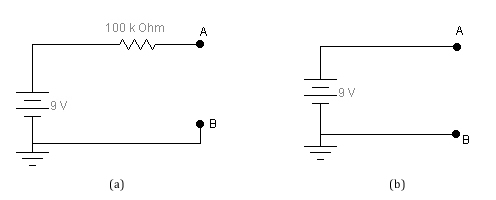
\includegraphics[width=0.66\textwidth]{images/p1-item-1.jpg}
	\caption{Estimación ideal de la caída de tensión entre\\ los bornes A y B de los circuitos (a) y (b).}
\end{figure}
\bigskip


	Adentrándonos en la parte experimental, pasaremos a medir la tensión sobre los bornes A y B de los circuitos de la \textit{Figura 2} utilizando un voltímetro analógico.
\bigskip

% Figura 2
\begin{figure}[h]
	\centering
	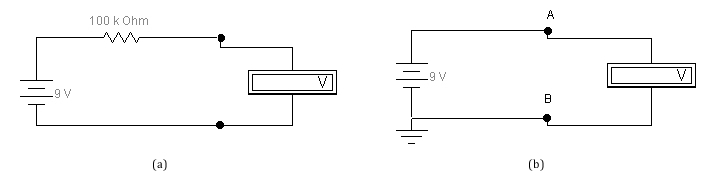
\includegraphics[width=0.94\textwidth]{images/p1-item-2.jpg}
	\caption{Medición empírica de la caída de tensión entre\\ los bornes A y B de los circuitos (a) y (b).}
\end{figure}
\bigskip


\noindent Habiendo utilizado el multímetro analógico \textit{TRIPLETT 630-APLK}, se obtuvieron los siguientes resultados:
\bigskip

	\indent \textbf{Circuito (a):} $V_{medido} = 6V$ \smallskip\\
	\indent \textbf{Circuito (b):} $V_{medido} = 8,6V$ \\
	\medskip

	Sin embargo, al reemplazar el instrumento analógico por uno digital (en nuestro caso se utilizó un multímetro digital \textit{UNI-T Modelo UT30F}) se obtuvieron los siguientes valores de tensión:
\bigskip

	\indent \textbf{Circuito (a):} $V_{medido} = 8,91V$ \smallskip\\
	\indent \textbf{Circuito (b):} $V_{medido} = 9,02V$ \\
	\bigskip



\newpage
	En las mediciones hechas con ambos multímetros se puede observar que con el multímetro analógico los valores de la tensión son más bajos que con el multímetro digital. Notar que en el \textbf{Circuito (a)} se aprecia una mayor diferencia en la tensión medida que en el \textbf{Circuito (b)}.
	\par
	Estas variaciones se deben a que las resistencias internas de los instrumentos son diferentes. Idealmente, estas resistencias internas son infinitas, de tal modo que por el voltímetro no pase corriente. Pero en la realidad, esto es imposible.
	\par
	Si miramos el \textbf{Circuito (a)}, en el mutímetro analógico se leyeron $6V$, mientras que en el multímetro digital se observaron $8,91V$. Como los multímetros están en serie con la fuente y la resistencia de 100k$\Omega$, a mayor resistencia interna del instrumento, menor va a ser la corriente que circula, y mayor el voltaje que lee el instrumento. En el caso del analógico, los $6V$ leídos significan que los otros $3V$ se perdieron en la resistencia de 100k$\Omega$. En cambio, con el digital sólo caen $0,09V$ en la resistencia, lo que significa que la corriente es menor en este caso, y el multímetro digital se acerca más que el analógico a lo ideal.
	\par
	Estos resultados reflejan la importancia de conocer la resistencia interna de los instrumentos que estamos utilizando para mesurar ya que, inevitablemente influirán en la precisión y exactitud de los datos de las variables que estamos midiendo.
\bigskip

% Figura 3
\begin{figure}[h]
	\centering
	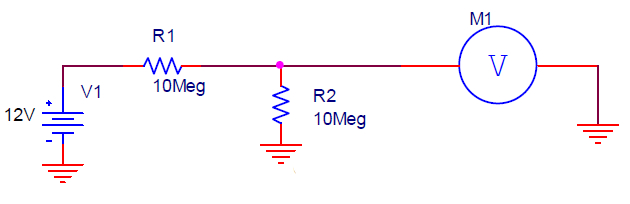
\includegraphics[width=0.85\textwidth]{images/p1-item-8.jpg}
	\caption{Circuito divisor de tensión.}
\end{figure}
\bigskip\bigskip


	Considerando ahora el circuito divisor de tensión de la \textit{Figura 3}\footnote{El valor de la tensión de la fuente es sólo como referencia, pero puede utilizarse cualquier otro razonable. En nuestro caso se mantuvieron los 12V propuestos.}, se medirá la tensión sobre la resistencia $R_2$ ubicada en el mismo. Si lo analizamos teóricamente, esperamos obtener una caída de tensión de 6V. La medición empírica se ha realizado con un voltímetro analógico y uno digital. Los valores obtenidos fueron:
\bigskip\medskip

\begin{tabular}{l l}
	\textbf{Multímetro analógico:} & $V_{medido} = 0,3V$ \smallskip\\
	\textbf{Multímetro digital:} & $V_{medido} = 3,9V$ \\
\end{tabular}
\bigskip\bigskip


\noindent Claramente hay una gran diferencia entre ambos instrumentos, siendo más alarmante la lectura dada por el multímetro analógico. Si nos remontamos a los resultados y conclusiones de las mediciones anteriores vemos que es muy lógico lo que acaba de ocurrir. El instrumento analógico, en función de voltímetro, posee una resistencia interna chica en comparación al valor del resistor \textit{R2}, por lo que, en el paralelo entre ambas predominará la primera de estas. De esta manera, la mayor caída de tensión se dará en la resistencia \textit{R1} ya que posee el mismo valor resistivo que \textit{R2}.
	\par
	Sin embargo, en el multímetro digital, también en su función de voltímetro, la resistencia interna es mayor a la presentada por el instrumento analógico. Esto hará que la lectura de tensión sea mayor, aunque seguirá siendo menor al valor ideal que espera obtenerse debido a que la resistencia interna sigue siendo menor al valor resistivo de \textit{R2}.
	\par
	Estos nuevos resultados confirman la significancia que tienen las resistencias internas provistas por los instrumentos.
\bigskip\bigskip




% DESARROLLO - PARTE 2
\subsection{Parte 2}

%% item (a)

	Se ha armado para el desarrollo de este apartado el circuito de medición mostrado en la \textit{Figura 4}. Hemos utilizado en esta ocación dos resistores cuyos valores están indicados como \textit{$R_1=100\Omega$} y \textit{$R_2=100k\Omega$}. Estos fueron colocados uno a la vez en el lugar representado en la figura como una resistencia \textit{R}. Las mediciones fueron realizadas con multímetros analógicos y también con digitales.
\bigskip

% Figura 4
\begin{figure}[h]
	\centering
	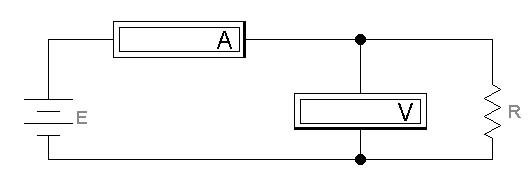
\includegraphics[width=0.72\textwidth]{images/p2-item-a.jpg}
	\caption{Circuito de medición.}
\end{figure}
\bigskip\bigskip


\noindent En la \textit{Tabla 2} se pueden observar los valores medidos y calculados para este circuito. Para el calculo de las resistencias \textit{R} se ha utilizado la \textit{Ley de Ohm}:
\medskip

\begin{equation}
 	R = {V \over I},
\end{equation}
\medskip

\noindent mientras que el \textit{error relativo porcentual} se calculó como la suma de los errores relativos de \textit{V} e \textit{I} multiplicado por 100.
\bigskip\bigskip


% Tabla 2
\begin{table}[!hbt]
	\begin{center}

		\begin{tabular}{|c|c|c|c|c|c|c|c|c|c|} \hline
			\multicolumn{5}{|c|}{\textbf{Multímetro digital}} & \multicolumn{4}{|c|}{\textbf{Multímetro analógico}} \\ \hline
			\multirow{5}{*}{\textbf{100$\Omega$}} 
			& \textbf{V} & \textbf{I} & \textbf{R} & \textbf{${\Delta R \over R}$} & \textbf{V} & \textbf{I} & \textbf{R} & \textbf{${\Delta R \over R}$} \\\cline{2-9}
			& V & mA & k$\Omega$ & \% & V & mA & k$\Omega$ & \% \\\cline{2-9}
			& 0.2 & 1.98 & 0.10101 &  & 0.2 & 1.2 & 0.16667 &  \\\cline{2-9}
			& 0.397 & 3.94 & 0.10076 &  & 0.4 & 3.2 & 0.125 &  \\\cline{2-9}
			& 0.601 & 5.96 & 0.10084 &  & 0.6 & 5.6 & 0.10714 &  \\ \hline
			\multirow{5}{*}{\textbf{100k$\Omega$}} 
			& \textbf{V} & \textbf{I} & \textbf{R} & \textbf{${\Delta R \over R}$} & \textbf{V} & \textbf{I} & \textbf{R} & \textbf{${\Delta R \over R}$} \\\cline{2-9}
			& V & mA & k$\Omega$ & \% & V & mA & k$\Omega$ & \% \\\cline{2-9}
			& 2 & 0.020 & 100 &  & 2 & 0.030 & 66.667 &  \\\cline{2-9}
			& 5 & 0.050 & 100 &  & 4 & 0.062 & 64.516 &  \\\cline{2-9}
			& 8 & 0.080 & 100 &  & 6 & 0.094 & 63.830 &  \\ \hline
		\end{tabular}

	\caption{Tabla de valores medidos y calculados para el\\ circuito de la Figura 4.}
	\end{center}
\end{table}
\bigskip



%% item (b)

	Hecho esto, se pasó a rearmar el circuito de manera de obtener la configuración mostrada en la \textit{Figura 5}. Nuevamente hemos utilizado dos resistores cuyos valores están indicados como \textit{$R_1=100\Omega$} y \textit{$R_2=100k\Omega$}. Estos fueron colocados uno a la vez en el lugar representado en la figura como una resistencia \textit{R}. Las mediciones fueron realizadas con multímetros analógicos y también con digitales.
\bigskip

% Figura 5
\begin{figure}[h]
	\centering
	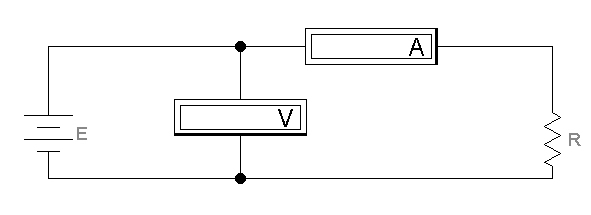
\includegraphics[width=0.78\textwidth]{images/p2-item-b.jpg}
	\caption{Circuito de medición.}
\end{figure}
\bigskip\bigskip


	En la \textit{Tabla 3} se pueden observar los valores medidos y calculados para este último circuito.
\bigskip


% Tabla 3
\begin{table}[!hbt]
	\begin{center}

		\begin{tabular}{|c|c|c|c|c|c|c|c|c|c|} \hline
			\multicolumn{5}{|c|}{\textbf{Multímetro digital}} & \multicolumn{4}{|c|}{\textbf{Multímetro analógico}} \\ \hline
			\multirow{5}{*}{\textbf{100$\Omega$}} 
			& \textbf{V} & \textbf{I} & \textbf{R} & \textbf{${\Delta R \over R}$} & \textbf{V} & \textbf{I} & \textbf{R} & \textbf{${\Delta R \over R}$} \\\cline{2-9}
			& V & mA & k$\Omega$ & \% & V & mA & k$\Omega$ & \% \\\cline{2-9}
			& 0.199 & 1.66 & 0.1199 &  & 0.2 & 1.0 & 0.2000 &  \\\cline{2-9}
			& 0.401 & 3.35 & 0.1197 &  & 0.4 & 2.6 & 0.1538 &  \\\cline{2-9}
			& 0.6 & 5.02 & 0.1195 &  & 0.6 & 4.4 & 0.1364 &  \\ \hline
			\multirow{5}{*}{\textbf{100k$\Omega$}} 
			& \textbf{V} & \textbf{I} & \textbf{R} & \textbf{${\Delta R \over R}$} & \textbf{V} & \textbf{I} & \textbf{R} & \textbf{${\Delta R \over R}$} \\\cline{2-9}
			& V & mA & k$\Omega$ & \% & V & mA & k$\Omega$ & \% \\\cline{2-9}
			& 2 & 0.020 & 100 &  & 2 & 0.020 & 100 &  \\\cline{2-9}
			& 5 & 0.050 & 100 &  & 4 & 0.040 & 100 &  \\\cline{2-9}
			& 8 & 0.080 & 100 &  & 6 & 0.062 & 96.774 &  \\ \hline
		\end{tabular}

	\caption{Tabla de valores medidos y calculados para el\\ circuito de la Figura 5.}
	\end{center}
\end{table}
\bigskip



%% item (c)

	Por último se midieron los resistores anteriores con los multimetros analógico y digitale respectivamente, en su función óhmetro. Las lecturas se encuentran volcadas sobre la \textit{Tabla 4}.


% Tabla 4
\begin{table}[!hbt]
	\begin{center}
	\begin{tabular}{|c|c|c|}
		\hline
		\textbf{Resistor} & \textbf{Multímetro digital} & \textbf{Multímetro analógico} \\
		\hline
		$R_1 (100\Omega)$ & $100.5\Omega$ & $85\Omega$ \\
		\hline
		$R_2 (100k\Omega)$ & $99.2k\Omega$ & $100k\Omega$ \\
		\hline
	\end{tabular}
	\caption{Valores de las resistencias medidas con los multímetros.}
	\end{center}
\end{table}



%% Cuestionario

\textit{¿Qué diferencias se observan entre las mediciones realizadas?}
\medskip

	[ Colocar respuesta aquí ]
\bigskip\bigskip


\textit{¿A qué factores se deben esas diferencia?}
\medskip

	[ Colocar respuesta aquí ]
\bigskip\bigskip


\textit{¿Qué influencia tendrá el tipo de conexión de los instrumentos?}
\medskip

	[ Colocar respuesta aquí ]
\bigskip\bigskip


\textit{¿Qué nombre se le ocurriría poner a cada tipo de conexión?}
\medskip

	[ Colocar respuesta aquí ]
\bigskip\bigskip


\textit{¿De qué manera se pueden aplicar los conceptos obtenidos en la parte (a) en la (b)?}
\medskip

	[ Colocar respuesta aquí ]
\bigskip\bigskip



% DESARROLLO - PARTE 3
\subsection{Parte 3}



% APÉNDICE

\newpage
\vspace*{4cm}
\begin{center}
	\textbf{\Huge{Apéndice}} \\
	\bigskip\bigskip
	\Large{\textit{``Hojas de datos de instrumentos de medición''}}
\end{center}

\end{document}
